\documentclass[12pt,letterpaper,english]{article}
\usepackage[utf8]{inputenc}
\usepackage[T1]{fontenc}
\usepackage[english]{babel}
\usepackage[letterpaper, margin=1in]{geometry}
\usepackage[pdftex]{graphicx}
\usepackage{fancyhdr}
\usepackage{setspace}
\usepackage{amsmath}
\usepackage{amsfonts}
\usepackage{commath}
\usepackage{lastpage}
\usepackage[usenames,dvipsnames,svgnames,table]{xcolor}
\usepackage{minted}
\usepackage{isodate}
\usepackage{hyperref}

\pagestyle{fancy}
\fancyhead{}
\fancyfoot{}
\fancyhead[HR]{\thepage\ of \pageref{LastPage}}

\DeclareMathSizes{12}{13}{8}{8} 
\DeclareMathOperator{\divf}{div}
\DeclareMathOperator{\jac}{jac}

\begin{document}


\begin{titlepage}
\thispagestyle{plain}
\begin{center}
\topskip0pt
\vspace*{\fill}

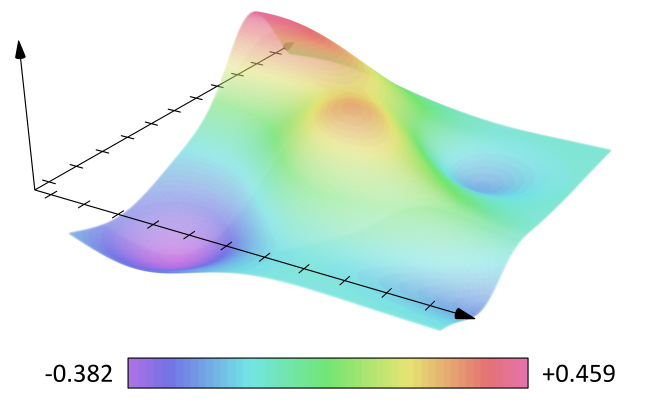
\includegraphics[width=3cm]{logo.png}\\[1cm]

\rule{\linewidth}{0.5mm}\\[0.5cm]

\textsc{\LARGE Visualizing functions of multiple variables}\\[1cm]

\textsc{\large By Sam Grayson and Wilson Nguyen}\\[0.7cm]

{\large \isodate}

\rule{\linewidth}{0.5mm}\\[1cm]

\vspace{0.9cm}

\end{center}

\section*{Abstract}

Visualizing the concepts of multivariable calculus can be challenging. The students created several computer-generated visual models utilizing the Mathematica language. These models can be used as teaching aids for educators or extra instruction for students.

\vspace*{\fill}

\end{titlepage}

\section*{Acknowledgements}

Thank you to Mrs. Harrelson for making a remarkable Multivariable Calculus class at LASA. This class is seriously the bomb if you like to think mathematically. We want to acknowledge the families of the students who have been incredibly supportive, even though they don't understand why we are doing this.

\tableofcontents

\clearpage

\doublespacing

\section{Introduction}

 As students, we know that visualizing these topics can sometimes be pretty difficult. I may or may not be guilty, on occasion, of simply using these formulas without an understanding of what they really do. If only there were some means of playing around with these topics without having to imagine clear mountains with magical rings or bleeding, toilet paper pasted shaved faces (inside joke). We believe that we have created the solution!

 The magic of Multivariable can be seen through the “Sam and Wilson’s 3D Multivariable Visualizer for Glazed-eyed LASA students” for a small fee of appreciation. The goals of this Visualizer are to allow students to interact with the topics discussed below and instead of telling the students  what the topics are, the Visualizer simply shows them. The topics would reveal themselves to even the most distant of students simply nodding their heads as asked (inside joke once more). We hope that you incorporate this Visualizer into your lessons and take advantage of the many opportunities that this opens up for students.

\section{Design Principles}

\begin{itemize}
\item \textbf{Flexibility:} The same concept can be visualized on multiple examples, and we tried to make it so that the models can adjust at runtime to any user inputted example.
\item \textbf{Interactivity:} The concepts are best illustrated when the user can tweak the values and adjust the parameters in a dynamic way that gives real-time feedback.
\item \textbf{Maintainability:} The models \textit{look good}. They are designed to be very clean and adjustable. This means that the code may be less aligned with the mathematics, but it is worth it for ease of maintaining. This way, when we graduate the models may still be adapted to the curriculum.
\item \textbf{Instructiveness:} The models are not by themselves. They are accompanied by text % TODO: in this paper?
explaining how they work and what they do.
\end{itemize}

\section{Frenet-Serret frames}

\subsection*{Overview}

The Frenet frame is a tool for understanding the local motion of a curve. The Frenet-Serret frame gives you an idea of where the function would be going if it were a straight line (tangent vector), which way the function would be bending if it were a circle (normal vector), and which way the function is twisting (binormal vector). Additional quantities like the curvature (related to the radius of the function if it were a circle) and the torsion (related to the angular momentum in the direction of the binormal vector). This visualization renders a video which shows the Frenet-Serret frame moving along a path. \cite{frenet1} \cite{frenet2} \cite{frenet3}

\subsection*{Theoretical basis}

The input should be a regular path in real space. \(c(t) : [a, b] \to \mathrm R^3\).

\begin{enumerate}
%\item Unit parametrize the curve. Let the arc-length passed up as a function of time given by \(s(t)\) \(s(t) = \int\limits_0^t \|f'(t)\|\). It can be shown that \(s(t)\) always has an inverse \(s^{-1}(t)\) (See the appendix for proof). Then let \(f(s^{-1}(t)) = c(t)\).
% TODO: link to appendix

%Since \(s'(t) = \|f'(t)\|\) by the fundamental theorem, and the length of a vector must be positive, the \(s(t)\) must be monotonically increasing. All monotonically increasing functions are injective. Taking \(\cod f = \im f\), it must also be surjective. Therefore \(s(t)\) is always invertible.

\item Calculate the unit tangent vector. Taylor's Theorem gives us \(c(t_0) + c'(t) \cdot (t - t_0) \approx c(t)\) for small \(\delta t\). A straight line starting at \(\vec{u}\) in the direction of \(\vec{v}\) is given by \(\vec{u} + \vec{v} \cdot t\). Therefore the line that locally approximates the function \(f\) is the first-order Taylor's Theorem. Since the tangent vector is relative to the point\(\vec{u} = \vec{0}\), and relative to the time \(t = 0\), and unit normalized, it is given by \(T(t) = \frac{c'(t)}{\|c'(t)\|}\).

\item Calculate the unit normal vector. Let \(c(t)\) be approximated by a circle of radius \(r\) lying in the plane spanned by \(T(0)\) and \(N(0)\) (this vector is not yet known). \(c(t) \approx r T(0) \sin t + r N(0) \cos t\). Then \(c'(t) = r T(0) \cos t - r N(0) \sin t\) (the reader can verify that at \(t = 0\), the tangent vector is indeed \(T(0)\)). Then \(c''(t) = T'(t) = - r T(0) \sin t - r N(0) \cos t\). Therefore \(T'(0) = -rN(0)\) which points in the direction of the normal vector. Therefore the unit-normalized normal vector is given by \(N(t) = \frac{T'(t)}{\|T'(t)\|}\). % TODO: get rid of negative sign

\item Calculate the curvature. \(\kappa(t) = \frac{1}{r}\) in the circle described by \(c(t) \approx r T(0) \sin t + r N(0) \cos t\). As previously shown, \(T'(0) = -r N(0)\). Therefore \(\frac{1}{\|T'(0)\|}\) gives the curvature.

% TODO: explain torsion

\item Calculate the binormal vector. In order to form an orthnormal basis, \(B(t) = T(t) \times N(t)\).

%\item Additionally, the Darboux vector can be computed. The Darboux vector is the angular velocity vector. The rate of rotation going from one vector to another is the cross-product between the vectors divided by the time it took to rotate. Therefore % TODO: complete this

\end{enumerate}

\subsection*{Implementation details}

There are multiple ways the Wolfram Language can compute derivatives. The first is \href{https://reference.wolfram.com/language/ref/D.html}{symbolically computing the derivative}. This calculates the answer using the variables. \(\frac{\dif}{\dif x}(3x^2)\) could be written \verb+D[3x^2, x]+ which evaluates to \verb+6x+. This expression can later be evaluated with a specific \verb+x+ for a numeric answer. The second is \href{http://reference.wolfram.com/language/NumericalCalculus/ref/ND.html}{numerically computing the derivative}. This method uses a very small change in the independent variable. \(\frac{\dif}{\dif x}(3x^2\mid_{x=5})\) could be written \verb+ND[3x^2, x, 5]+ evaluates to \verb+30+. There are functions like the absolute value which don't have symbolic derivatives, but do have numeric derivatives. It is also about ten times faster. Therefore, for this program I used the numeric derivative.

All of the important quantities are given as a function of \verb+t+. This is because it makes animation easier if arbitrary inputs can be supplied. First the user enters a path as a function of \verb+t+. Then the tangent vector (based on the path), the normal vector (based on the tangent vector), and the binormal vector (based on the tangent and normal vectors) are calculated as described in previous subsection. The curvature is calculated based on the tangent vector, as described in the previous subsection.

After that each quantity described above must be rendered as a 3D-graphic. The output is put into a single frame. Outputs from different points along the path are put into a list. That list gets animated by the built-in \href{https://reference.wolfram.com/language/ref/ListAnimate.html}{ListAnimate}.

\subsection*{Usage notes}

This program could be used to create a video demonstrating the Frenet-Serret frames in preparation for a lecture (not real-time). This video could be displayed after slide 4 of lecture 6 (Motion in 3 space). It would provide a visualization for what the Frenet-Serret frame represents.

\begin{enumerate}
\item Change \verb+pathF[t_] = ...+ to be whatever path you want in terms of \verb+t+.
\item Change \verb+tmin+ and \verb+tmax+ to span the domain of the path.
\item Evaluate the cell with Shift+Enter. You should see a the path appear below. Tweak any of the above values if necessary.
\item Evaluate each cell until you hit the bottom with Shift+Enter. It may take up to twenty minutes to render the video.
\item When completed, the Wolfram Language should display a file name in the last cell. The video is located there.
\end{enumerate}


\section{Scalar field and friends}

\subsection*{Overview}

A scalar field \(f\) from \(\mathbb R^2 \to \mathbb R\) can be visualized by a surface in three dimensions. On this surface, the x-traces and y-traces can be shown as strings lying on the surface. The partial-derivatives can be show as vector stangent to each trace. The gradient is a vector that points in the direction of steepest descent. Level sets can be depicted as lines going around the surface. It can be noted visually that the gradient is always perpendicular to the level set. \cite{field6}

\subsection*{Theoretical Basis}

This time, the maths are relatively straightforward.

% The level set locally is given at the point 

\subsection*{Implementation details}

We created seven different virtual objects. In order to demonstrate the fact that gradient vectors point in the direction of greatest descent, we generated \verb+gradFieldR+ and overlaid it upon the graph of a scalar field, \verb+fieldR+, using \href{https://reference.wolfram.com/language/ref/Plot3D.html}{Plot3D}. The surface is semi translucent in order to be able to view the slices of x and y as separate functions. Next, we revealed that the gradients are always perpendicular to the level sets by using a mesh function in order to display slices of the function at varying values of Z that are constant along each slice. The x-trace is done by holding y constant. This creates the parametric \verb+{x, ymid, field /. y-> ymid}+ as a function of \verb+x+. This is rendered with \href{https://reference.wolfram.com/language/ref/ParametricPlot3D.html}{ParametricPlot3D}. Then the vector $\langle 1, 0, \frac{\partial f}{\partial x} \rangle$ is depicted eminating from $\langle x, y, f(x, y) \rangle$. The x partial is green and the y is red. Finally, the gradient is drawn from a point on the graph that is evaluated from.

\subsection*{Usage notes}

This model can be used to demonstrate topics that we learned in both the second and third six weeks of multivariable. Students will no longer have to worry about imaginary mountains demonstrations with this visual included in lectures. The slices no longer have to be silly putty or moon sand in the shape of functions, but instead actual 2-dimensional functions displayed on the graph. Any point and any surface can be chosen to displayed, all the calculations will be automatic, and the vectors will always be generated (except for at singularities if they exist).

These visualizations can be used in lectures 11 Partial Derivatives,12, Derivatives continued, and 15 Gradients and Directional Derivatives

\begin{enumerate}
\item The variable \verb+fieldF+ is the scalar valued function that can be altered to fit any function of your choice. 
\item \verb+xmin, xmax, ymin, ymax+ are the domain boundaries which can also be changed to preference.
\item \verb+xint, yint+ represents the increments for the display of the gradient vector field (also known as the spacing between the vectors).
\item \verb+xmid, ymid+ are the point at which the gradient vector, x partial, y partial, and x and y slices are calculated and displayed at. 
\item All of these variables are free to edit and the program will accommodate to new models of choice. 
\end{enumerate}

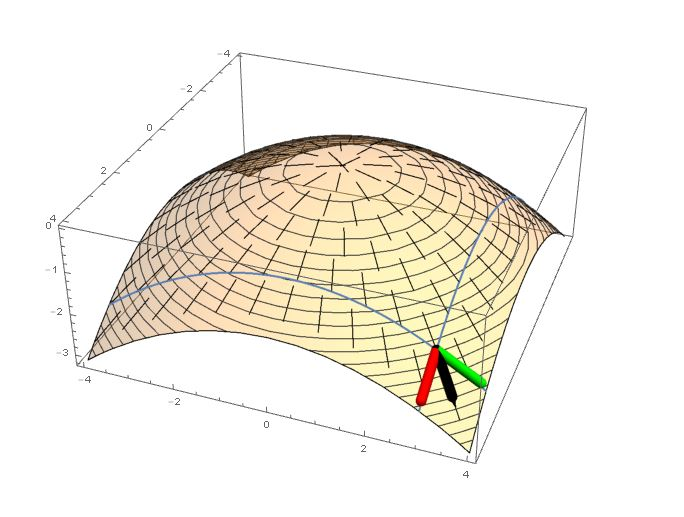
\includegraphics[height=10cm]{../exhibit/field.jpg}

%%% Local Variables:
%%% mode: latex
%%% TeX-master: "main"
%%% End:


\section{Change of variables}

\subsection*{Overview}

Change of variables is a technique by which a region of integration can be transformed into a different region, which may be easier to integrate over. This  transformation can be visualized as `stretching' space itself from one coordinate system to another. The caveat is that it might change the area of the region. Therefore, the integral must be scaled by the Jacobian.

\subsection*{Theoretical basis}

Take the parallelpiped spanned by \(h \langle \vec i, \vec j \rangle\) centered around \(\vec 0\). Notice that it has area \(h^2\). After applying transformation \(T : \mathbb R^3 \to \mathbb R^3\), we need to measure the volume of the new parallelpiped. For sufficiently small \(h\), \(T(h \vec i) = T(\vec 0) + h \frac{\partial T}{\partial x}\) by Taylor's Theorem. In the same way, \(T(h \vec j) = T(\vec 0) + h \frac{\partial T}{\partial y}\). Therefore the transformed parallelpiped is spanned by \(h \frac{\partial T}{\partial x}\) and \(\frac{\partial T}{\partial y}\). Remember \(T(\vec v) = \langle T_1(\vec v), T_2(\vec v) \rangle\) and \(\frac{\partial T}{\partial x} \in \mathbb R^2\). The area contained in the parallelpiped becomes \(h^2 \frac{\partial T}{\partial x} \times \frac{\partial T}{\partial y}\), which is exactly \(h^2 \jac T\).

\subsection*{Implementation details}

To make the animation, I have to take a weighted average between the original region and the final region where the weight on the original region decreases with time and the weight on the final region increases with time. In order to make this work out, the input must not be regions, but the boundaries of those regions represented as paths. Let the boundary of the first region be \verb+c[t]+ and the transformation of a vector \verb+v+ be described by the function \verb+transform[v]+. Each frame is \verb;c[t] * u + transform[c[t]] * (1 - u); where \verb+u+ varies with time.

The desired duration and number of frames is inputted in the program. The progrma precalculates each frame before rendering the animation, for efficiency. The animation can be played back in the Wolfram Language notebook, or it can be saved as a file.

\subsection*{Usage notes}

Unless you feel confident in programming, don't modify the paths. If you do feel confident, paths is a flattened list of parametric equations.  The transform is also tricky, but it takes on vector \verb+v+ and manipulates its components to create the transformed vector.

Because of the technical difficulty and computation time assoscaited it is recommended to leave everything in the default case. In the default case, they generate grid-lines in Polar and wheel-and-spokes in Cartesian. This has already been generated and the notebook does not need to be rerun. Simply play the \verb+change_of_variables.avi+ animation in any media player.

This animation fits in Lecture 26 Change of Variables Part 2 after slide 8 or slide 13.x

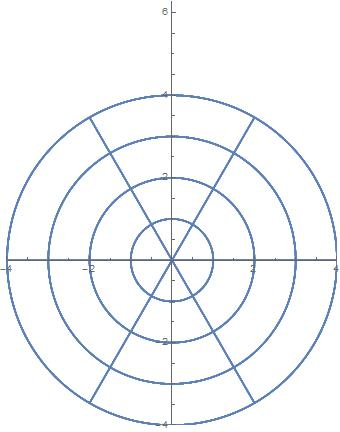
\includegraphics[width=0.2\textwidth]{../exhibit/change1.jpg}
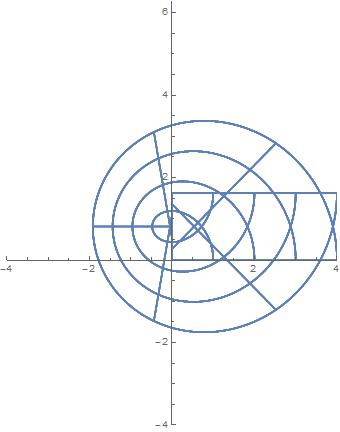
\includegraphics[width=0.2\textwidth]{../exhibit/change2.jpg}
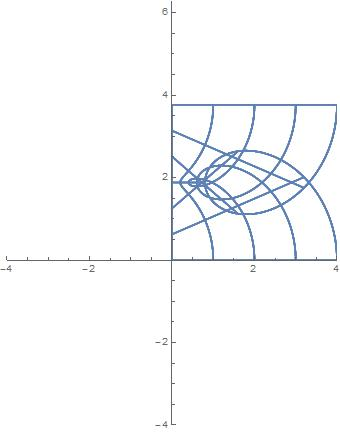
\includegraphics[width=0.2\textwidth]{../exhibit/change3.jpg}
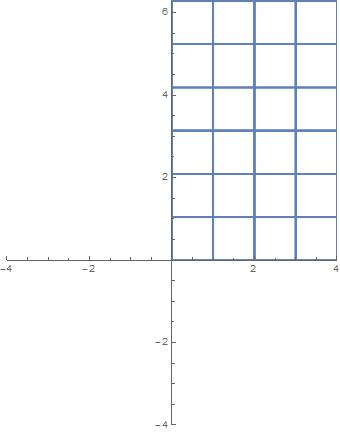
\includegraphics[width=0.2\textwidth]{../exhibit/change4.jpg}

%%% Local Variables:
%%% mode: latex
%%% TeX-master: "main"
%%% End:


\section{Flux Integral}

\subsection*{Overview}

Integrals over surfaces are difficult to visualize. There are scalar surface integrals which multiply the field by the surface area at each point on the surface, and there are vector surface integrals which measure the flux through that surface. These visualizations show the meaning of the surface tangent vectors \(T_u\) and \(T_v\). They also show the meaning of a flux integral of a vector field through a surface visually.

\subsection*{Implementation details}

This section is split into two visuals: one for scalar and one for vector fields. 

\textbf{Scalar surface integrals:} A 3D  plot is created using the scalar function of choice. The x partial and y partial are displayed using the vectors Then the vector $\langle 1, 0, \frac{\partial f}{\partial x} \rangle$ is depicted eminating from $\langle x, y, f(x, y) \rangle$. The cross product is produced by the vector $\langle \frac{\partial f}{\partial x}, \frac{\partial f}{\partial y}, 1 \rangle$. The x partial is green, the y is red, the cross product is blue. All of these are meshed using a mesh function and displayed as a single visual. \cite{flux8}

\textbf{Vector flux Integrals:} A 3D parametric function is displayed using the function \verb+param[u_, v_] =+ \verb+{Cos[u]*Sin[v],+ \verb+Sin[u]*Sin[v]+, \verb+Cos[v]}+ which of course in this example is the unit sphere. However, other parameterized surfaces can be chosen. The nice thing about using \verb+parametricPlot3D+ is level sets of u and v are also displayed on the surface. The u partials are the vectors \verb+{D[param[u, v][[1]], u],+ \verb+D[param[u, v][[2]], u],+ \verb+D[param[u, v][[3]], u]}+ which of course is the derivative of the parameterization based upon u and the v partial is calculated similarly except with respect to v. The u partial is red and the v is green. The normal is calculated by the the negative of the cross product of both partials in order to receive the outward facing normal. The vector field we chose for this demonstration was an interesting one: \verb+{Cos[u]^2/2, Sin[v]^3/2, Sin[u]*Cos[v]}+ which we overlaid and calculated only for the surface. Of course, any vector field may be chosen. The surface is semi-translucent to provide students the ability to look inside the parameterized surface. \cite{flux7}

\subsection*{Usage notes}

These models fully demonstrate all the parts needed to understand the components of these integrals. The surfaces, the partials, and the vector and scalar fields are all demonstrated in an easy to intuit manner. The models are incredibly customizable and will serve as practical means of demonstrating the concepts. 

These visualizations can be incorporated into lecture 31 Integrating over a Surface - Scalar valued functions and lecture 32 Surface Integrals (Flux).

\textbf{Scalar Surface Integrals:}
\begin{enumerate}
\item \verb+fieldF+ is the chosen scalar function.
\item \verb+xmin, xmax, ymin, ymax+ are the bounds of the domain.
\item \verb+xmid, ymid+ are the coordinates at which the partials and normal vector are calculated
\item All of these variables are free to edit and the program will accommodate to new models of choice
\end{enumerate}

\textbf{Vector-field Surface Integrals:}
\begin{enumerate}
\item \verb+umin, umax, vmin, vmax+ are the bounds of the parameters chosen. 
\item \verb+umid, vmid+ represent the coordinates at which the partials and the normal are calculated.
\item \verb+vectorincrementdensity+ is the increment in which the vectors are calculated along the surface. In simpler terms, a smaller number is a more detailed field and a bigger is a less detailed field. 
\item \verb+vectorfield+ is the the vector field that is chosen. 
\item All of these variables are free to edit and the program will accommodate to new models of choice
\end{enumerate}

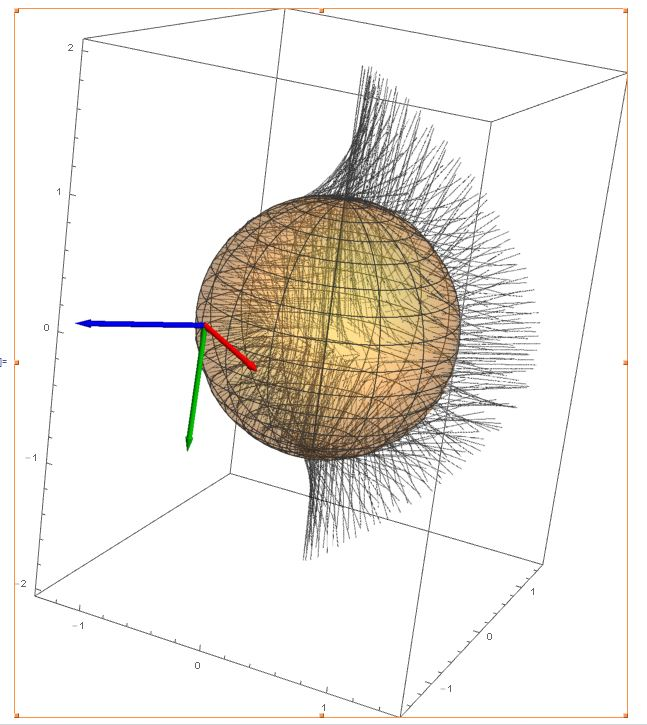
\includegraphics[height=10cm]{../exhibit/flux.jpg}

%%% Local Variables:
%%% mode: latex
%%% TeX-master: "main"
%%% End:


\section{Divergence}

\subsection*{Overview}

A vector field has divergence when the vectors in that field point away from some point. Point-charges are a real-world example of this. We created a visualization of the electric field created by point charges to visually depict divergence. The field in the visualization has zero divergence everywhere except for where the point-charges lie. \cite{divergence1} \cite{divergence2}

\subsection*{Theoretical basis}

Given a vector field \(\vec E : \mathbb R^3 \to \mathbb R^3\), divergence \(\divf \vec E\) or \(\nabla \cdot \vec E\) is defined as \(\frac{\partial E_x}{\partial x} + \frac{\partial E_y}{\partial y} + \frac{\partial E_z}{\partial z}\). This describes whether the field \(E\) is a source or a sink.

Two point-charges attract by Coulomb's Law \(\vec F = \frac{1}{4 \pi \epsilon_0} \frac{q_1 q_2}{\|r\|^3} \;\vec r\). Let the first charge \(q_1\) be called the source and the second charge \(q_2\) the test-charge. Observe that \(\vec F = q_2 \vec E\), where \(E = \frac{1}{4 \pi \epsilon_0} \frac{q_1}{\|r\|^3} \;\vec r\). This field \(\vec E\) is useful because it abstracts out the test-charge. The field is only dependent on the source and the position.

When the source is centered around the origin, \(\vec E(x, y, z) = \frac{1}{4 \pi \epsilon_0 (x^2+y^2+z^2)^{3/2}} \; \langle x, y, z \rangle\). Since \(\frac{\partial E_x}{\partial x}\) is given by the quotient rule as \(\frac{-2x^2+y^2+z^2}{4 \pi \epsilon_0 (x^2+y^2+z^2)^{5/2}}\), \(\frac{\partial E_y}{\partial y}\) and \(\frac{\partial E_z}{\partial z}\) are similar, then the divergence at any point off of the origin is given by: \(\divf \vec E = \frac{1}{4 \pi \epsilon_0} \frac{(-2x^2 + y^2 + z^2) + (x^2 - 2y^2 + z^2) + (x^2 + y^2 - 2z^2)}{4 \pi \epsilon_0 (x^2 + y^2 + z^2)^{5/2}} = \vec 0\). For the origin, the divergence is undefined.

But it is given by Maxwell's equations that \(\iiint_S \divf \vec E \cdot \dif V = \frac{q}{\epsilon_0}\). Since \(\divf \vec E\) is zero everywhere except at the origin, and the integral is non-zero, the origin must be a Delta-Dirac function. A Delta-Dirac function \(\sigma (x)\) is defined such that \(\sigma (x) = 0\) everywhere except at \(x = 0\), when \(\sigma(x)\) is undefined, and \(\int_{-\infty}^\infty \sigma(x) \dif x = 1\).  Therefore \(\divf \vec E (0, 0, 0) = \frac{q}{\epsilon_0} \sigma(x)\sigma(y)\sigma(z)\), where \(\sigma(x)\) is the Delta-Dirac function.

Therefore electric fields have zero divergence except for at the point-charge which causes them. At that point, the divergence is infinite. The integral of the divergence of the electric field over a surface is just the number of charges contained in that surface.

\subsection*{Implementation details}

The electric fields are scaled by \(\frac{4 \pi \epsilon_0}{q}\), so that these constants do not appear in any part of the code.

The electric fields are generated from a curried function. A curried function is a function that returns another function. In this case, the \verb+field+ function inputs the location of a point-charge and outputs a function of \verb+x+, \verb+y+, and \verb+z+ which represents the vector field.

The actual vector arrows, if care is not taken, will be very large around the point-charge. This is because the point-charge creates a singularity where the magnitude of the electric field goes to infinity. To mitigate this, we ignore the vectors that are right near the point-charge and only plot the ones that are a certain distance away. This is done by the \verb+restrict+ function.

\subsection*{Usage notes}

This is intended to show students what divergence actually means. It doesn't just mean that the vector field is expanding, because in this vector field divergence is zero even though the arrows are going farther apart. The arrows are also getting smaller in length, which cancels out their expansion. The only divergence is caused by the point-charge itself, which has infinite divergence. This could be introduced at Lecture 34 Vector Fields and Curl after slide 7 which can give a more nuanced explanation to divergence.

It can also show Gauss' Law. Since \(\iiint_S \divf \vec E \dif \vec V\) is simply the number of point-charges, the left-hand side of Gauss' Law simplifies to the total charge \(q_T\) in \(q_T = \iint_{\partial S} \vec E \cdot \dif \vec S\). Instead of taking a volume-integral of divergence, you can literally count the number of point charges (count up for positive charges and down for negative ones). As such this animation could be revisited at Lecture 37 Gauss' Theorem as a motivating example before starting the presentation.

\begin{enumerate}
\item Set \verb+restriction[point_, radiusofrestriction_]+ to ignore the singularity.
\item Adjust \verb+opacity+ for viewing prefrences. It changes the transparency of the bounding sphere. 
\item Place point charges as a function of \verb+u+.
\item Set the bounds of \verb+u+ to be suitable to the function.
\end{enumerate}

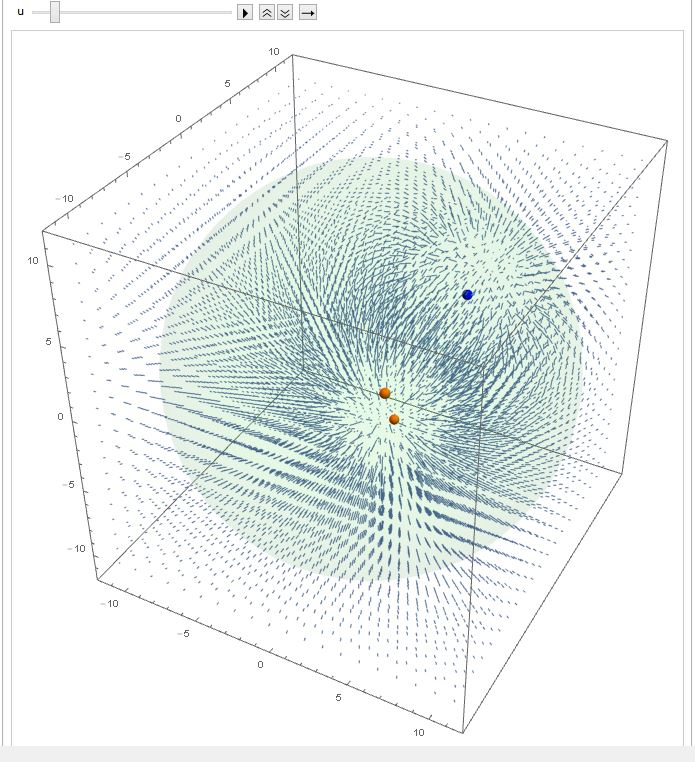
\includegraphics[height=16cm]{../exhibit/divergence.jpg}

%%% Local Variables:
%%% mode: latex
%%% TeX-master: "main"
%%% End:


\section{Bibliography}

\begin{thebibliography}{56}

\bibitem{frenet1}
  Weisstein, Eric W. ``Frenet Formulas.'' From \emph{MathWorld}--A Wolfram Web Resource. \url{http://mathworld.wolfram.com/FrenetFormulas.html}.

\bibitem{frenet2}
  Knisley, Jeff. ``Torsion and the Frenet Frame.'' \emph{Multivariable Calculus Online.} East Tennessee State University, 2001. \url{http://math.etsu.edu/multicalc/prealpha/Chap1/Chap1-8/part4.htm}.

\bibitem{frenet3}
  Sullivan, Michael. ``Frenet-Serret formulas and Torsion.'' \emph{Math 251.} Southern Illinois University. \url{http://galileo.math.siu.edu/mikesullivan/Courses/251/S11/torsion.pdf}

\bibitem{divergence1}
  Fitzpatrick, Richard. ``Gauss' Law'' \emph{Classical Electromagnetism.} University of Texas, 2006. \url{http://farside.ph.utexas.edu/teaching/em/lectures/node30.html}

\bibitem{divergence2}
  Duxbury, Phil. ``PHY481 - Lecture 2: Vector Calculus.'' \emph{Computational Physics for PHY481.} Michigan State University, 2009. \url{http://www.pa.msu.edu/~duxbury/courses/phy481/Fall2009/Lecture2.pdf}

\bibitem{field6}
  Azad, Kalid. ``Vector Calculus: Understanding the Gradient.'' BetterExplained.com. BetterExplained Inc, n.d. Web. 03 June 2015. \url{http://betterexplained.com/articles/vector-calculus-understanding-the-gradient/}

\bibitem{flux7}
  Nycamp, Duane Q. ``Introduction to a Sufrface Integral of a Vector Field.'' Mathinsight.org. Math Insight, n.d. Web. 03 June 2015. \url{http://mathinsight.org/surface_integral_vector_field_introduction}

\bibitem{flux8}
  Dawkins, Paul. ``Pauls Online Notes : Calculus III - Surface Integrals.'' Math.lamar.edu. Paul Dawkins, n.d. Web. 03 June 2015. \url{http://tutorial.math.lamar.edu/Classes/CalcIII/SurfaceIntegrals.aspx}

\end{thebibliography}

\end{document}

%%% Local Variables:
%%% mode: latex
%%% TeX-master: t
%%% End:
